%!TEX root = ../template.tex
%%%%%%%%%%%%%%%%%%%%%%%%%%%%%%%%%%%%%%%%%%%%%%%%%%%%%%%%%%%%%%%%%%%%
%% appendix1.tex
%% NOVA thesis document file
%%
%% Chapter with example of appendix with a short dummy text
%%%%%%%%%%%%%%%%%%%%%%%%%%%%%%%%%%%%%%%%%%%%%%%%%%%%%%%%%%%%%%%%%%%%

\typeout{NT FILE appendix_images.tex}%

\prependtographicspath{{Chapters/Figures/}}

% epigraph configuration
\epigraphfontsize{\small\itshape}
\setlength\epigraphwidth{12.5cm}
\setlength\epigraphrule{0pt}

\appendix
\chapter{Imagens}
\label{chp:imagens}

\section{Problema de \textit{Makespan}}

\begin{figure}[H]
	\centering
	\begin{subfigure}{0.49\textwidth}
	\centering
		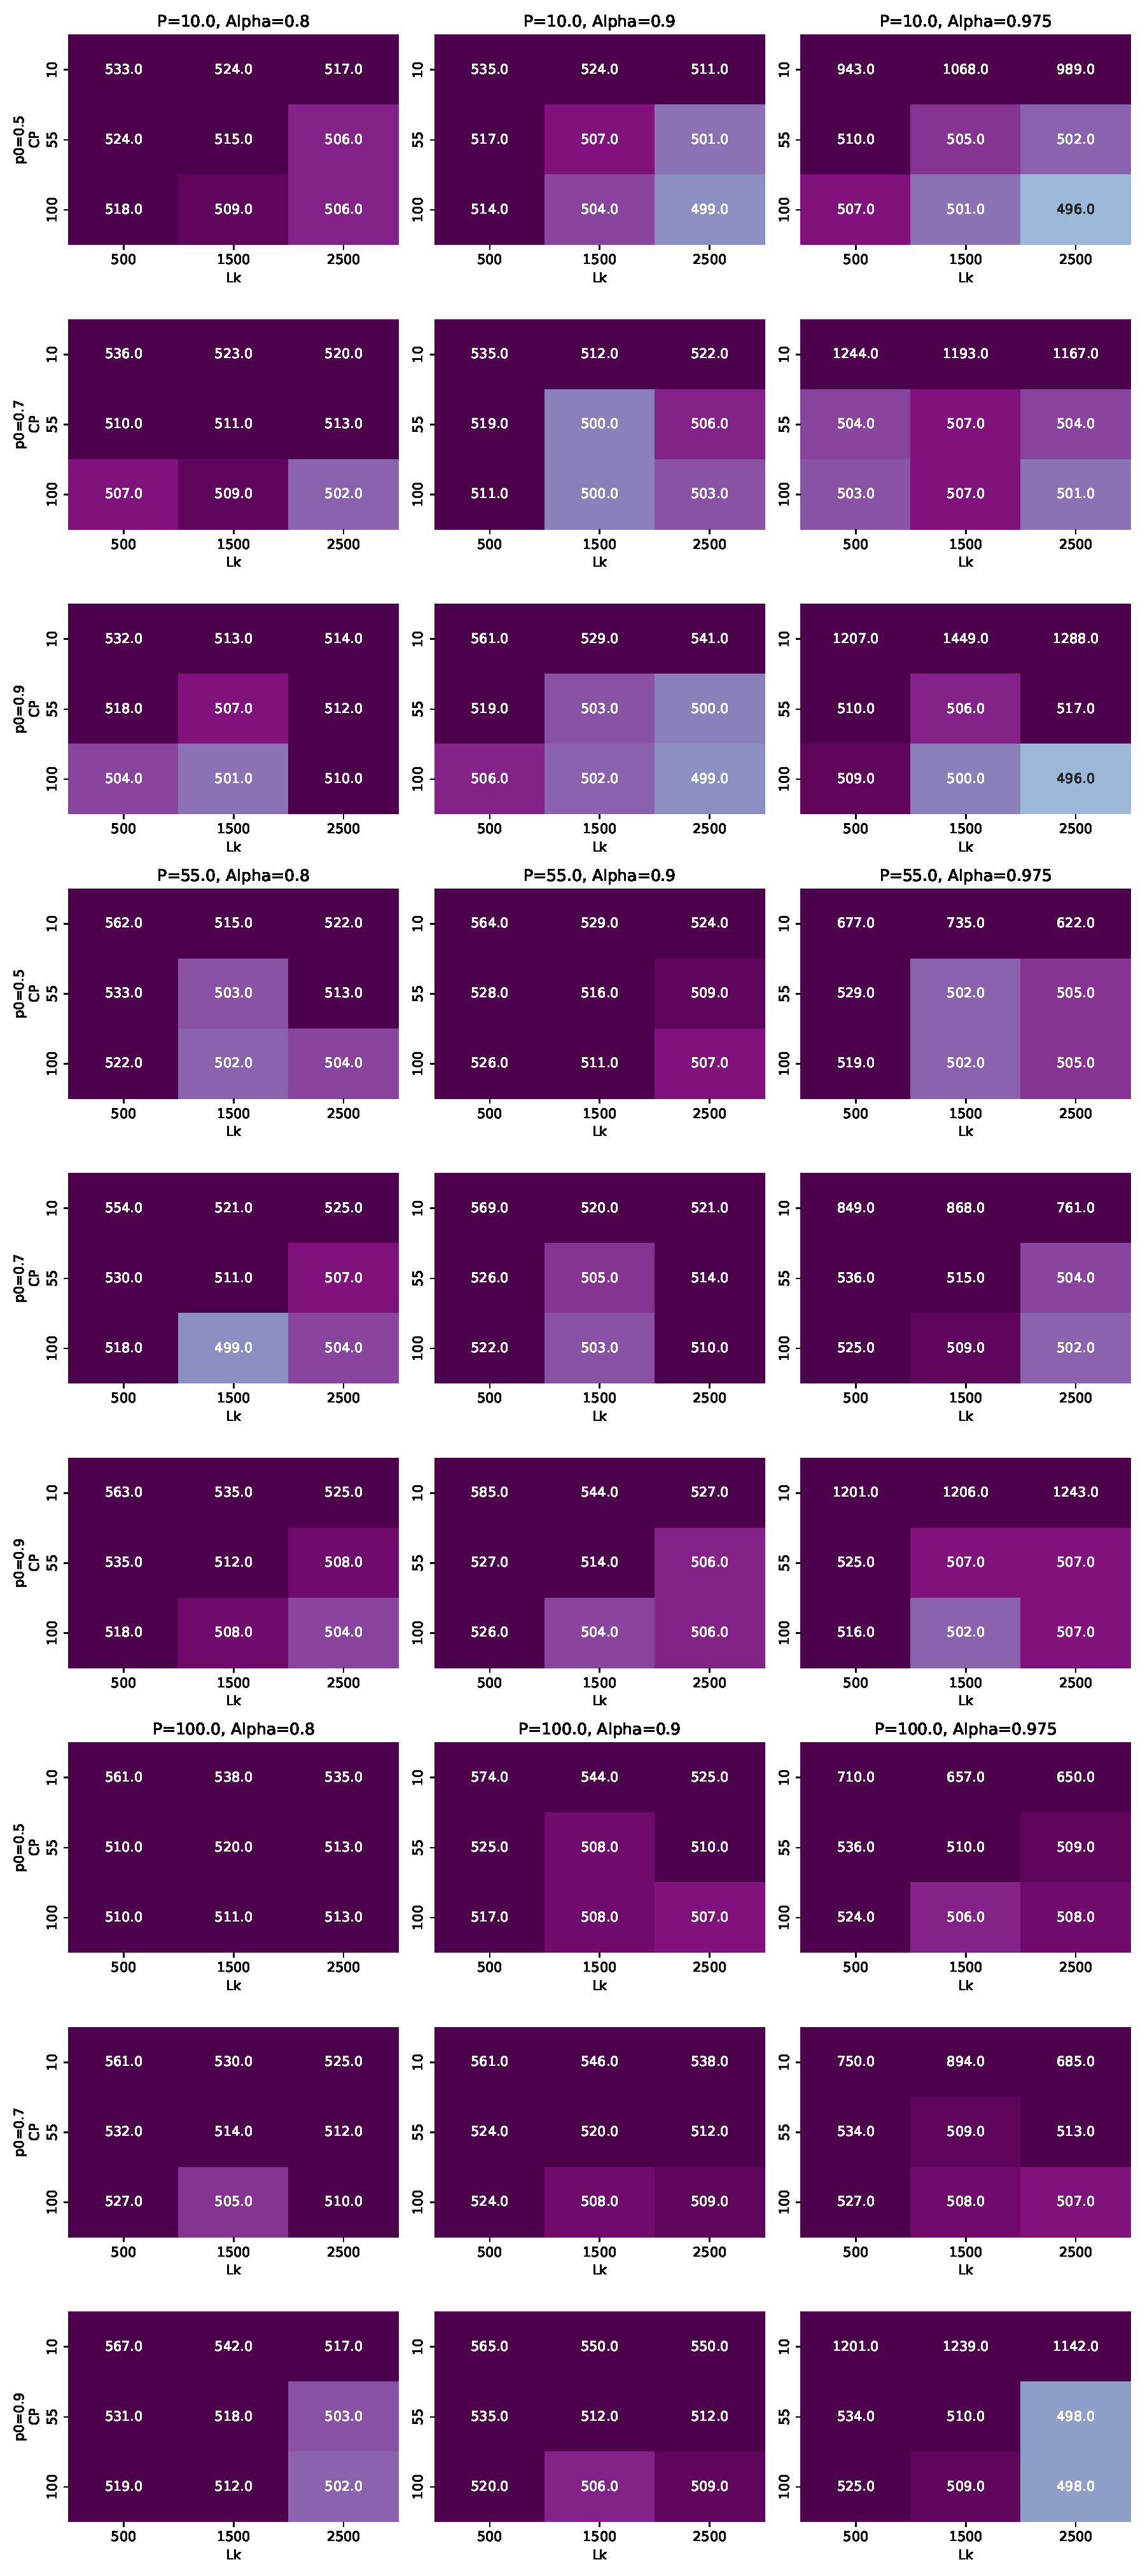
\includegraphics[width = \textwidth]{P1M1_NGV_best}
		\caption{Melhor \textit{makespan}}
		\label{fig:P1M1_NGV_best}
	\end{subfigure}
	\begin{subfigure}{0.49\textwidth}
	\centering
		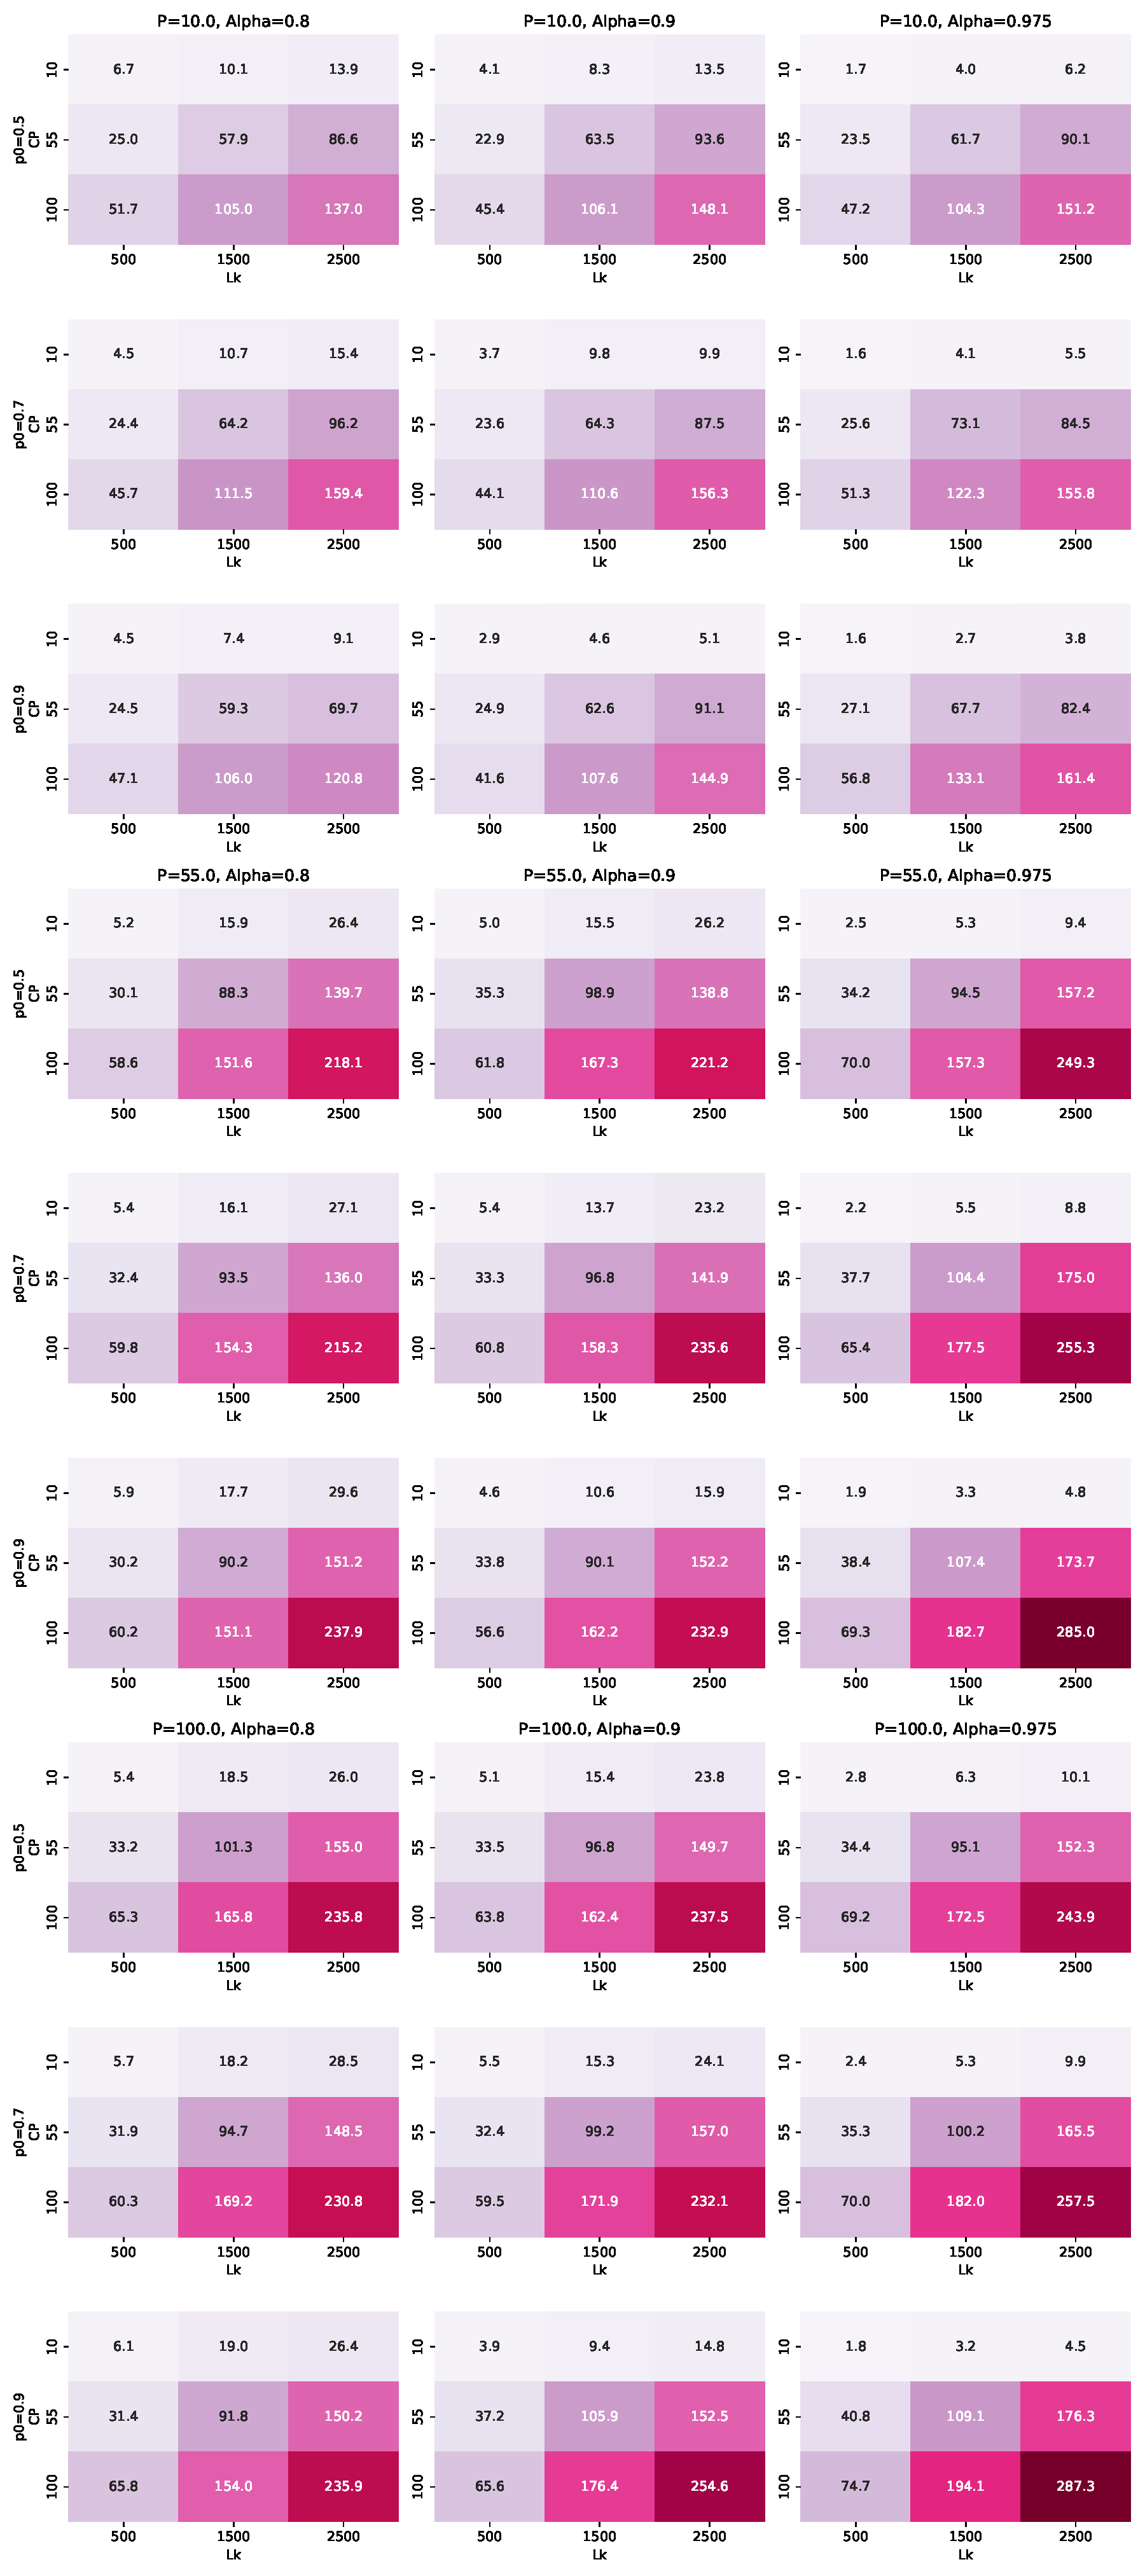
\includegraphics[width = \textwidth]{P1M1_NGV_runtime}
		\caption{Tempo de computação total}
		\label{fig:P1M1_NGV_runtime}
	\end{subfigure}
	\caption{Impacto dos níveis das variáveis sobre o valor da função objetivo e do tempo computacional para o modelo 1.}
	\label{fig:P1M1_NGV_alt}
\end{figure}

\begin{figure}[H]
	\centering
	\begin{subfigure}{0.49\textwidth}
	\centering
		\includegraphics[width = \textwidth]{P1M1_GV_best}
		\caption{Melhor \textit{makespan}}
		\label{fig:P1M1_GV_best}
	\end{subfigure}
	\begin{subfigure}{0.49\textwidth}
	\centering
		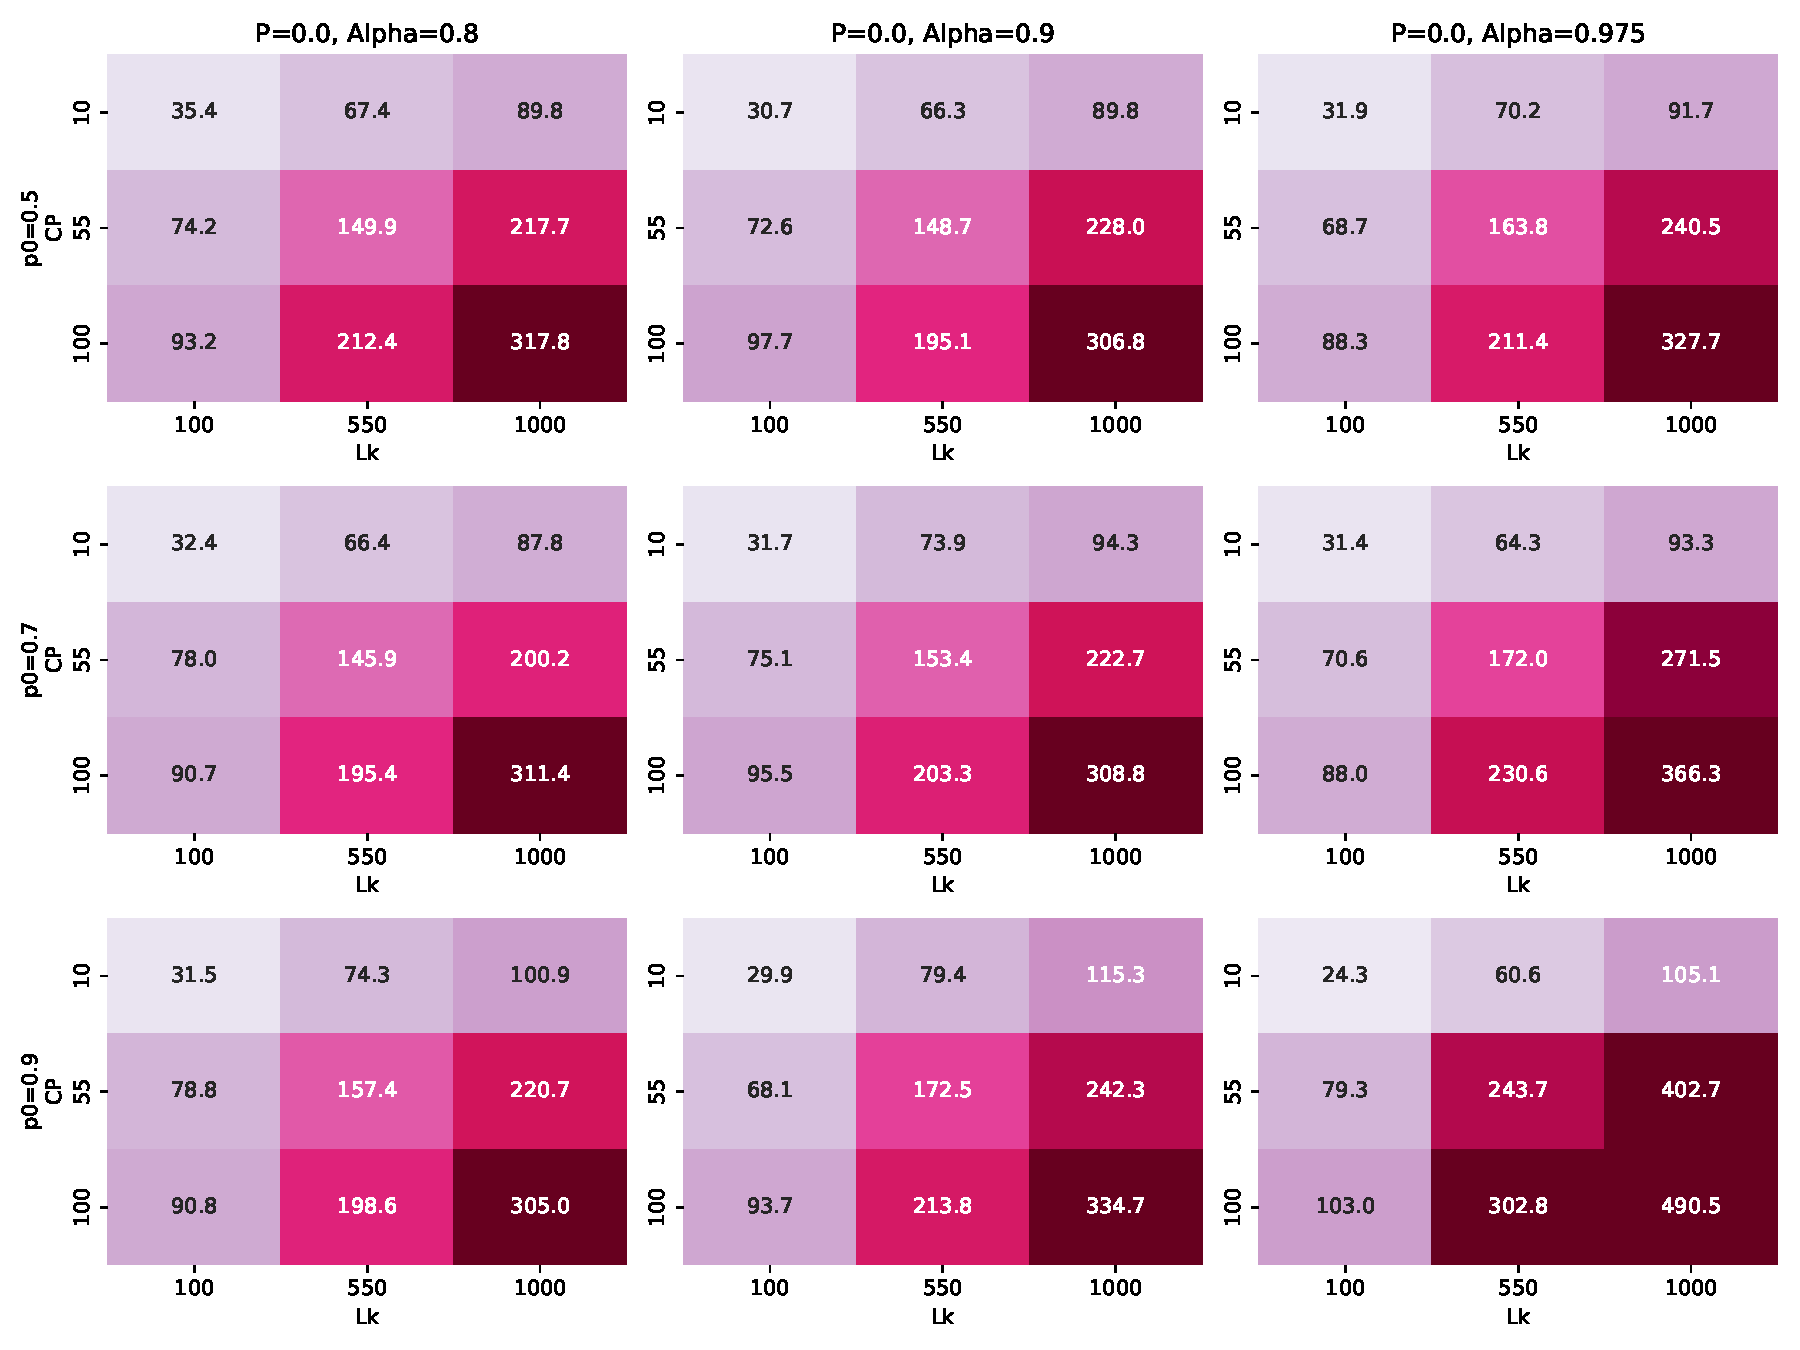
\includegraphics[width = \textwidth]{P1M1_GV_runtime}
		\caption{Tempo de computação total}
		\label{fig:P1M1_GV_runtime}
	\end{subfigure}
	\caption{Impacto dos níveis das variáveis sobre o valor da função objetivo e do tempo computacional para o modelo 2.}
	\label{fig:P1M1_GV_alt}
\end{figure}

\begin{figure}[H]
	\centering
	\begin{subfigure}{0.49\textwidth}
	\centering
		\includegraphics[width = \textwidth]{P1M2_GV_best}
		\caption{Melhor \textit{makespan}}
		\label{fig:P1M2_GV_best}
	\end{subfigure}
	\begin{subfigure}{0.49\textwidth}
	\centering
		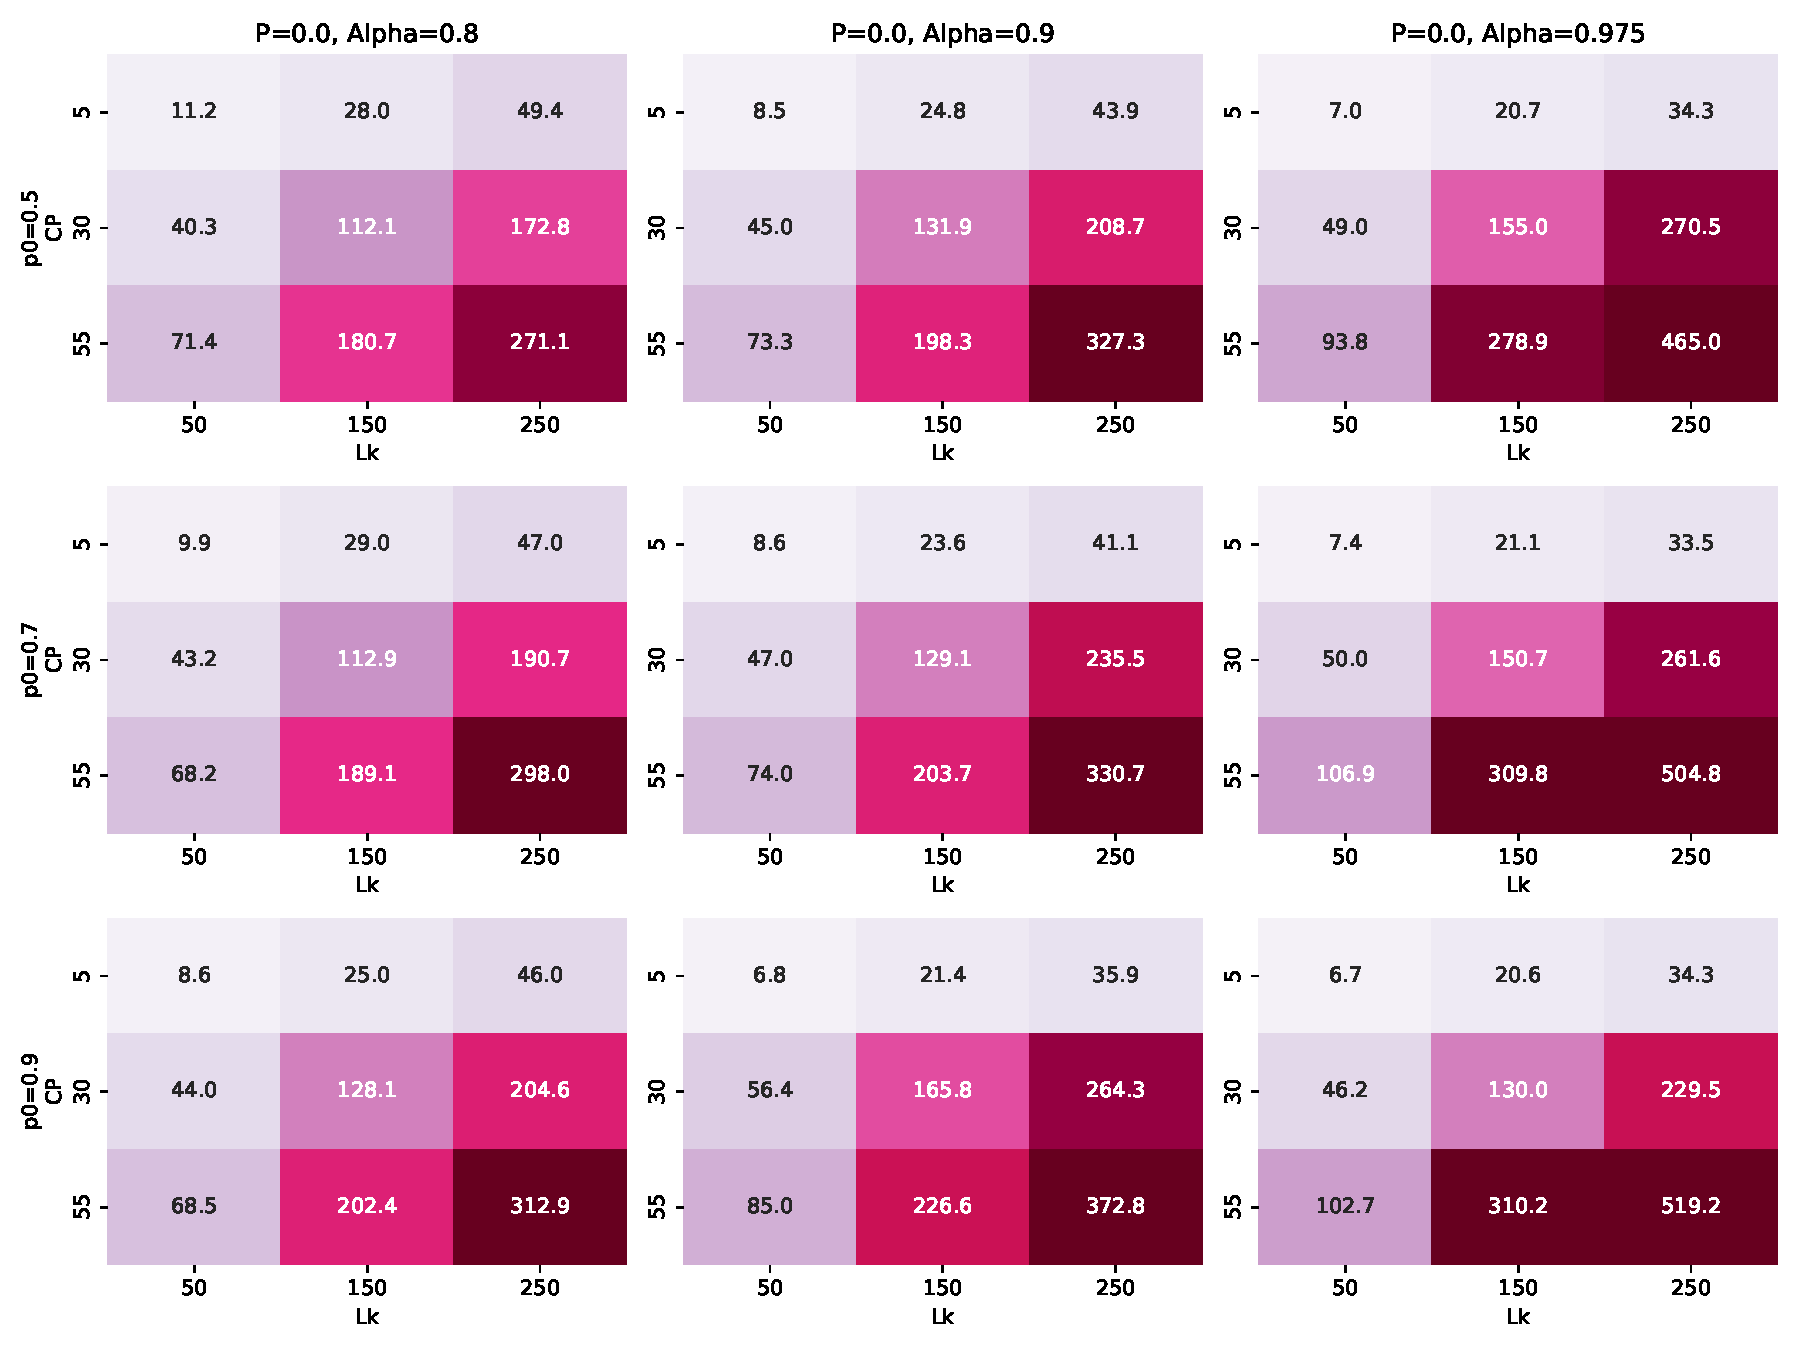
\includegraphics[width = \textwidth]{P1M2_GV_runtime}
		\caption{Tempo de computação total}
		\label{fig:P1M2_GV_runtime}
	\end{subfigure}
	\caption{Impacto dos níveis das variáveis sobre o valor da função objetivo e do tempo computacional para o modelo 3 com \textit{left shifting}.}
	\label{fig:P1M2_GV_alt}
\end{figure}

\begin{figure}[H]
	\centering
	\begin{subfigure}{0.49\textwidth}
	\centering
		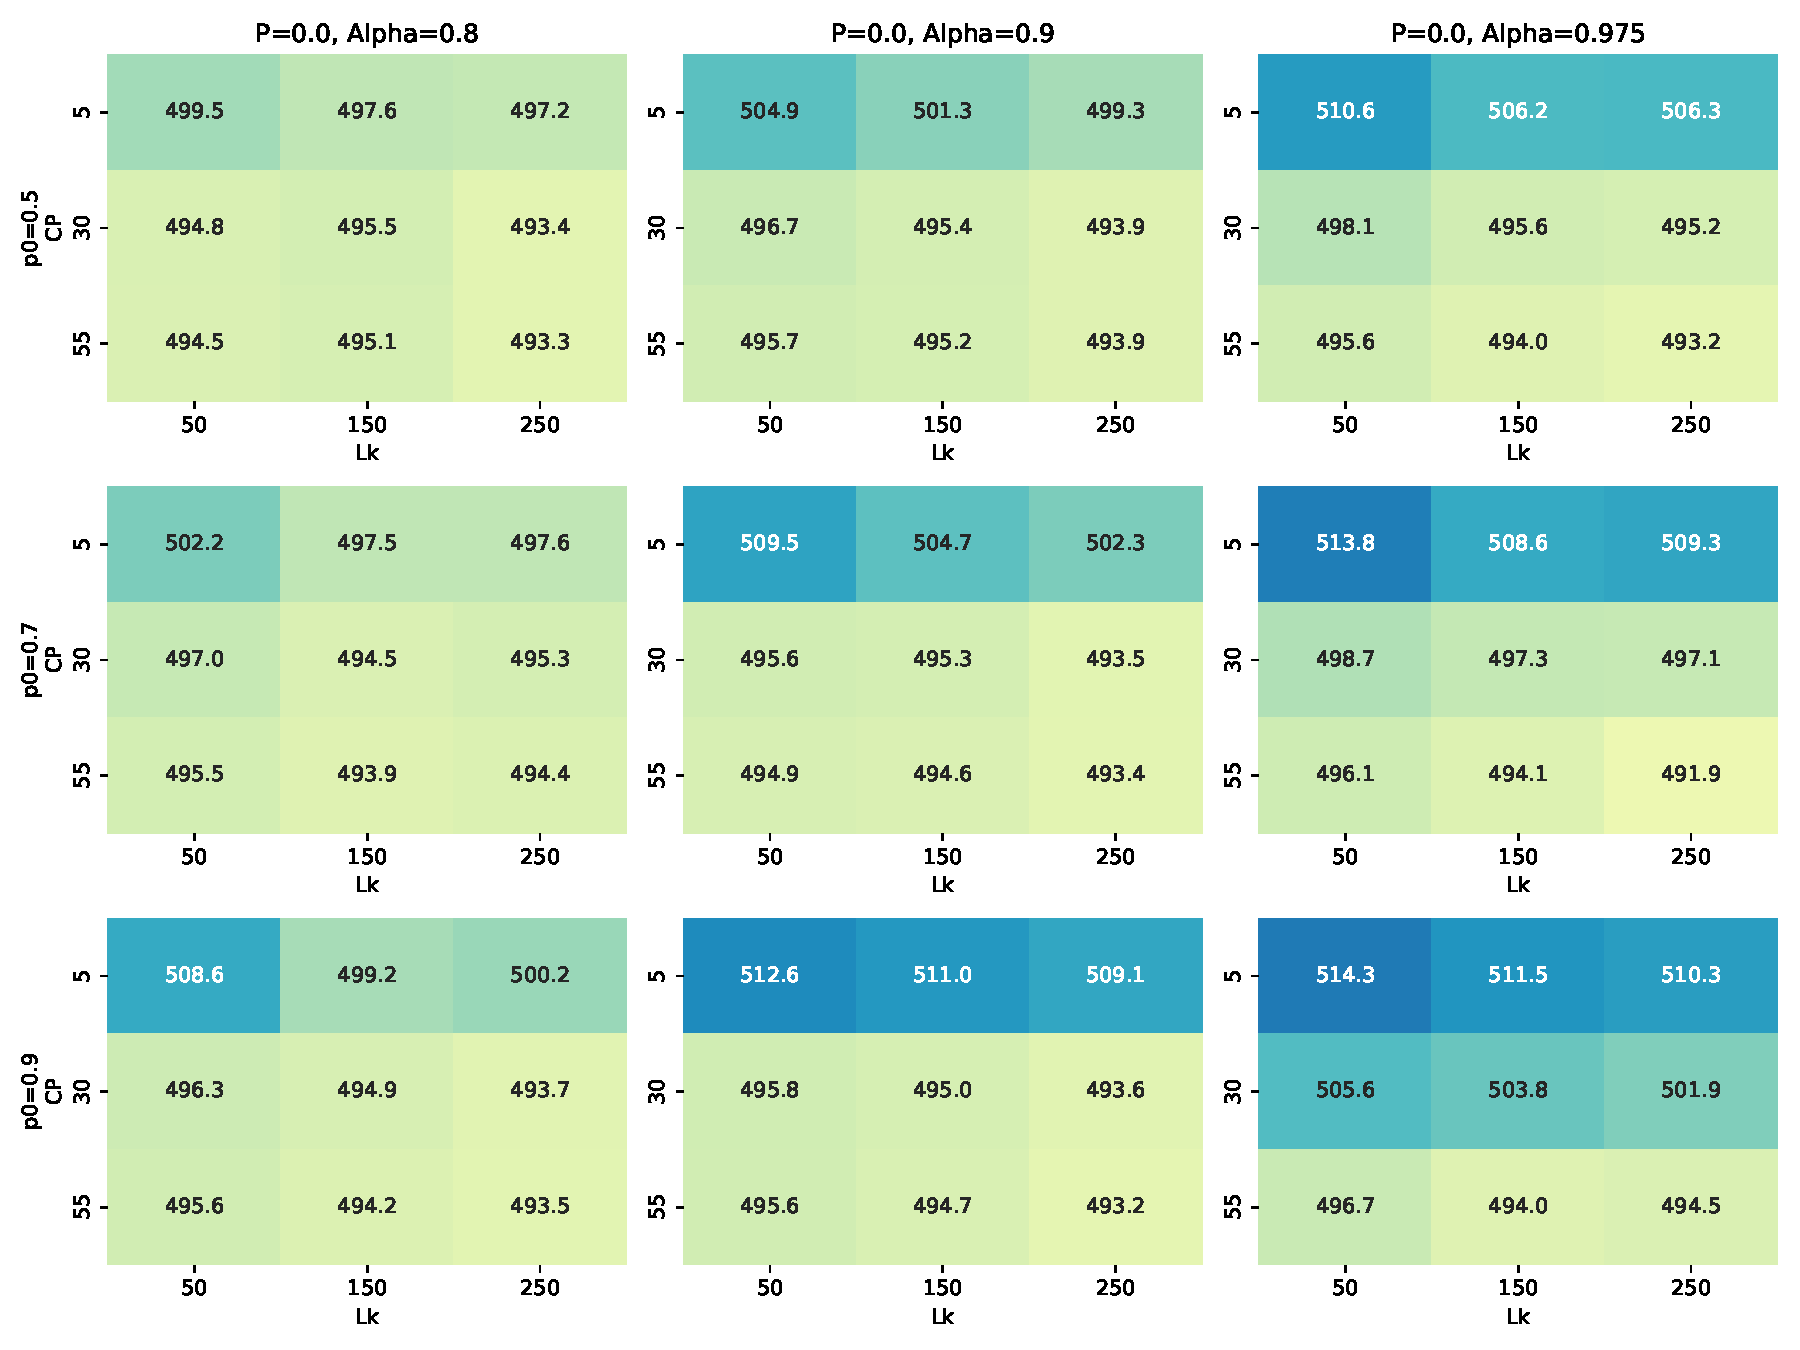
\includegraphics[width = \textwidth]{P1M2_GV_REVTT_objf}
		\caption{Média do mínimo de \textit{makespan}}
		\label{fig:P1M2_GV_REVTT_objf}
	\end{subfigure}
	\begin{subfigure}{0.49\textwidth}
	\centering
		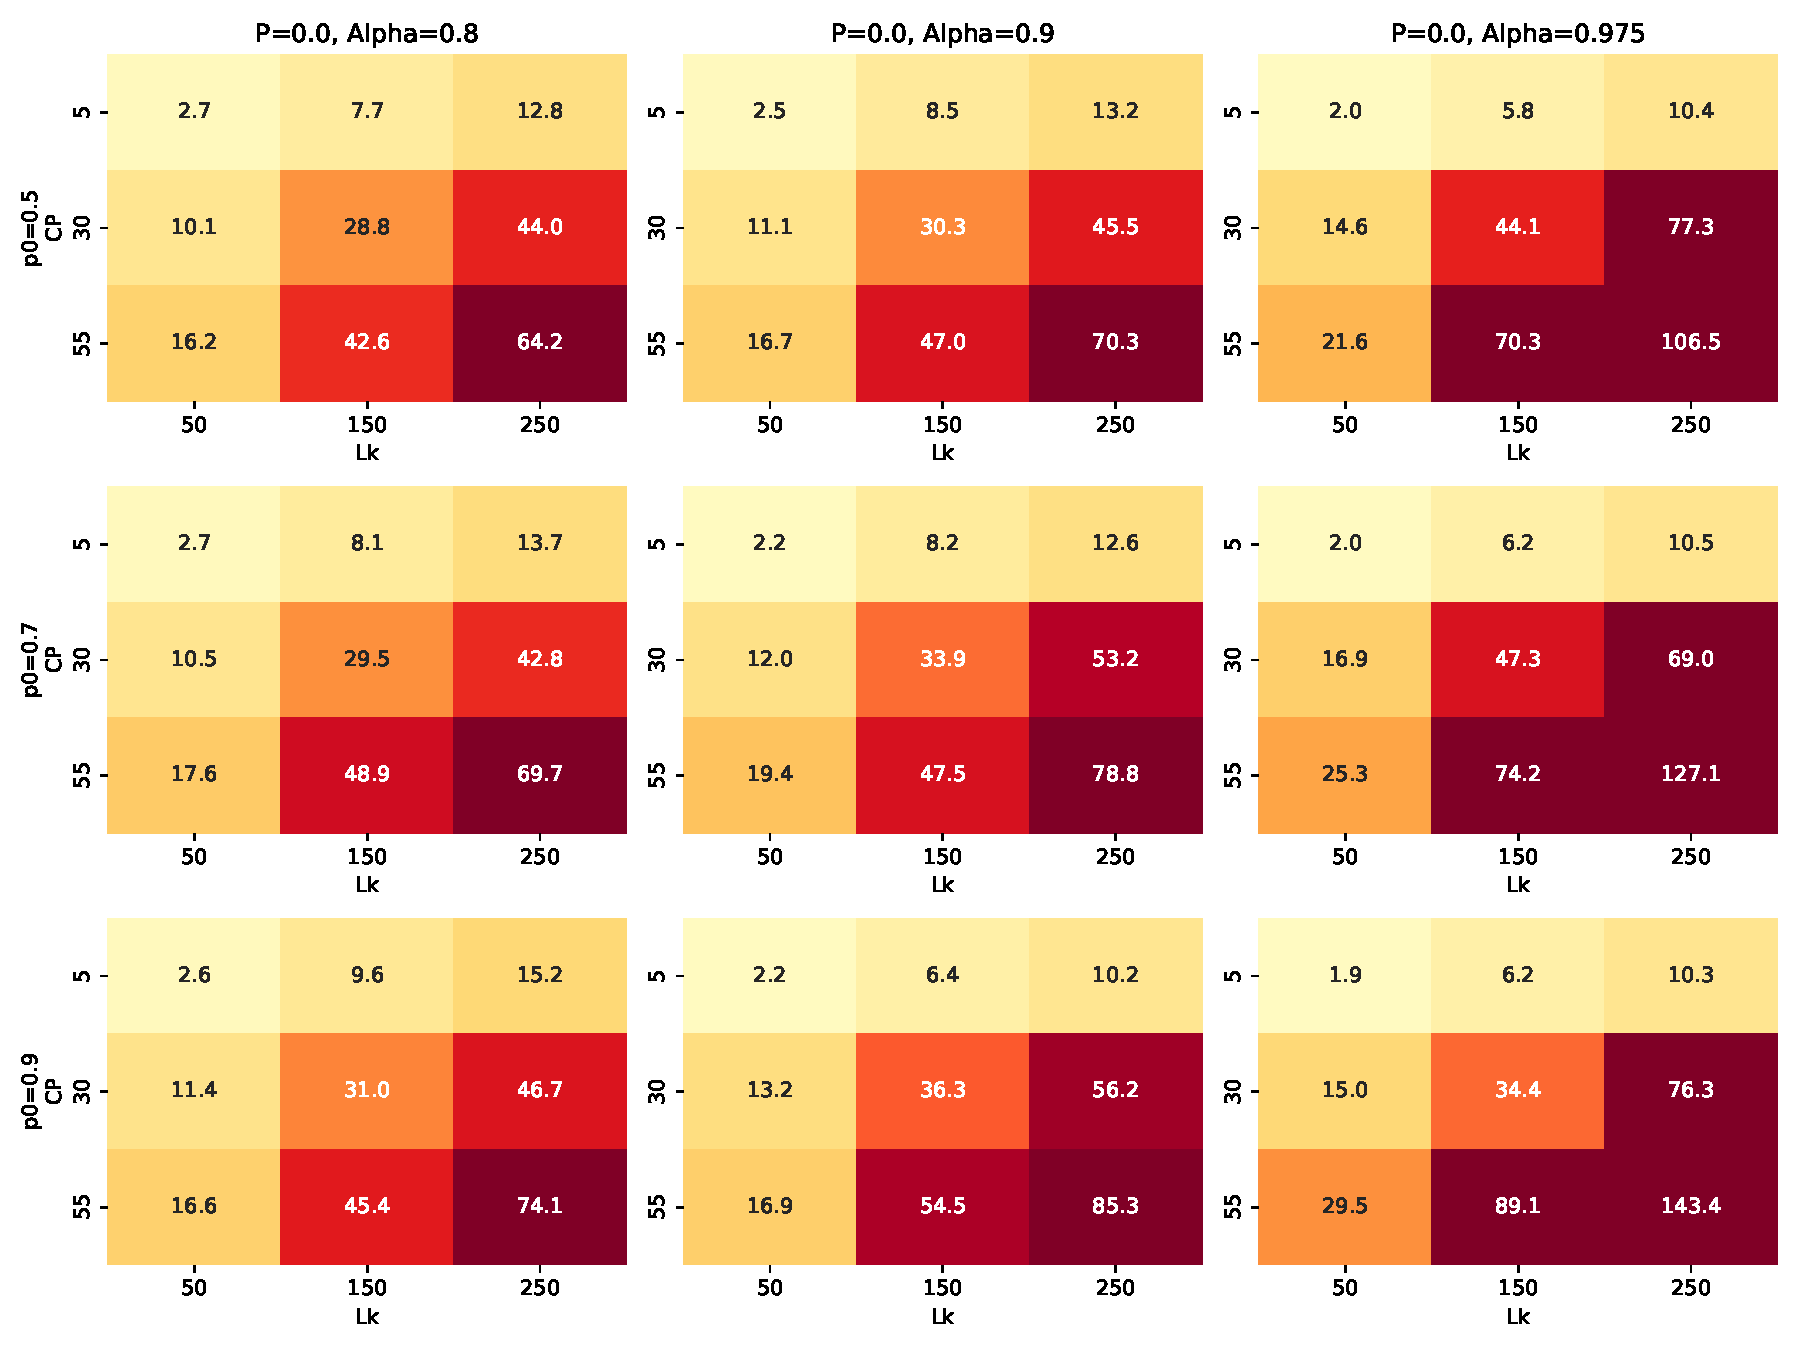
\includegraphics[width = \textwidth]{P1M2_GV_REVTT_time}
		\caption{Média do máximo do tempo de computação}
		\label{fig:P1M2_GV_REVTT_time}
	\end{subfigure}
	\label{fig:P1M2_GV_REVTT_alt}
	\centering
	\begin{subfigure}{0.49\textwidth}
	\centering
		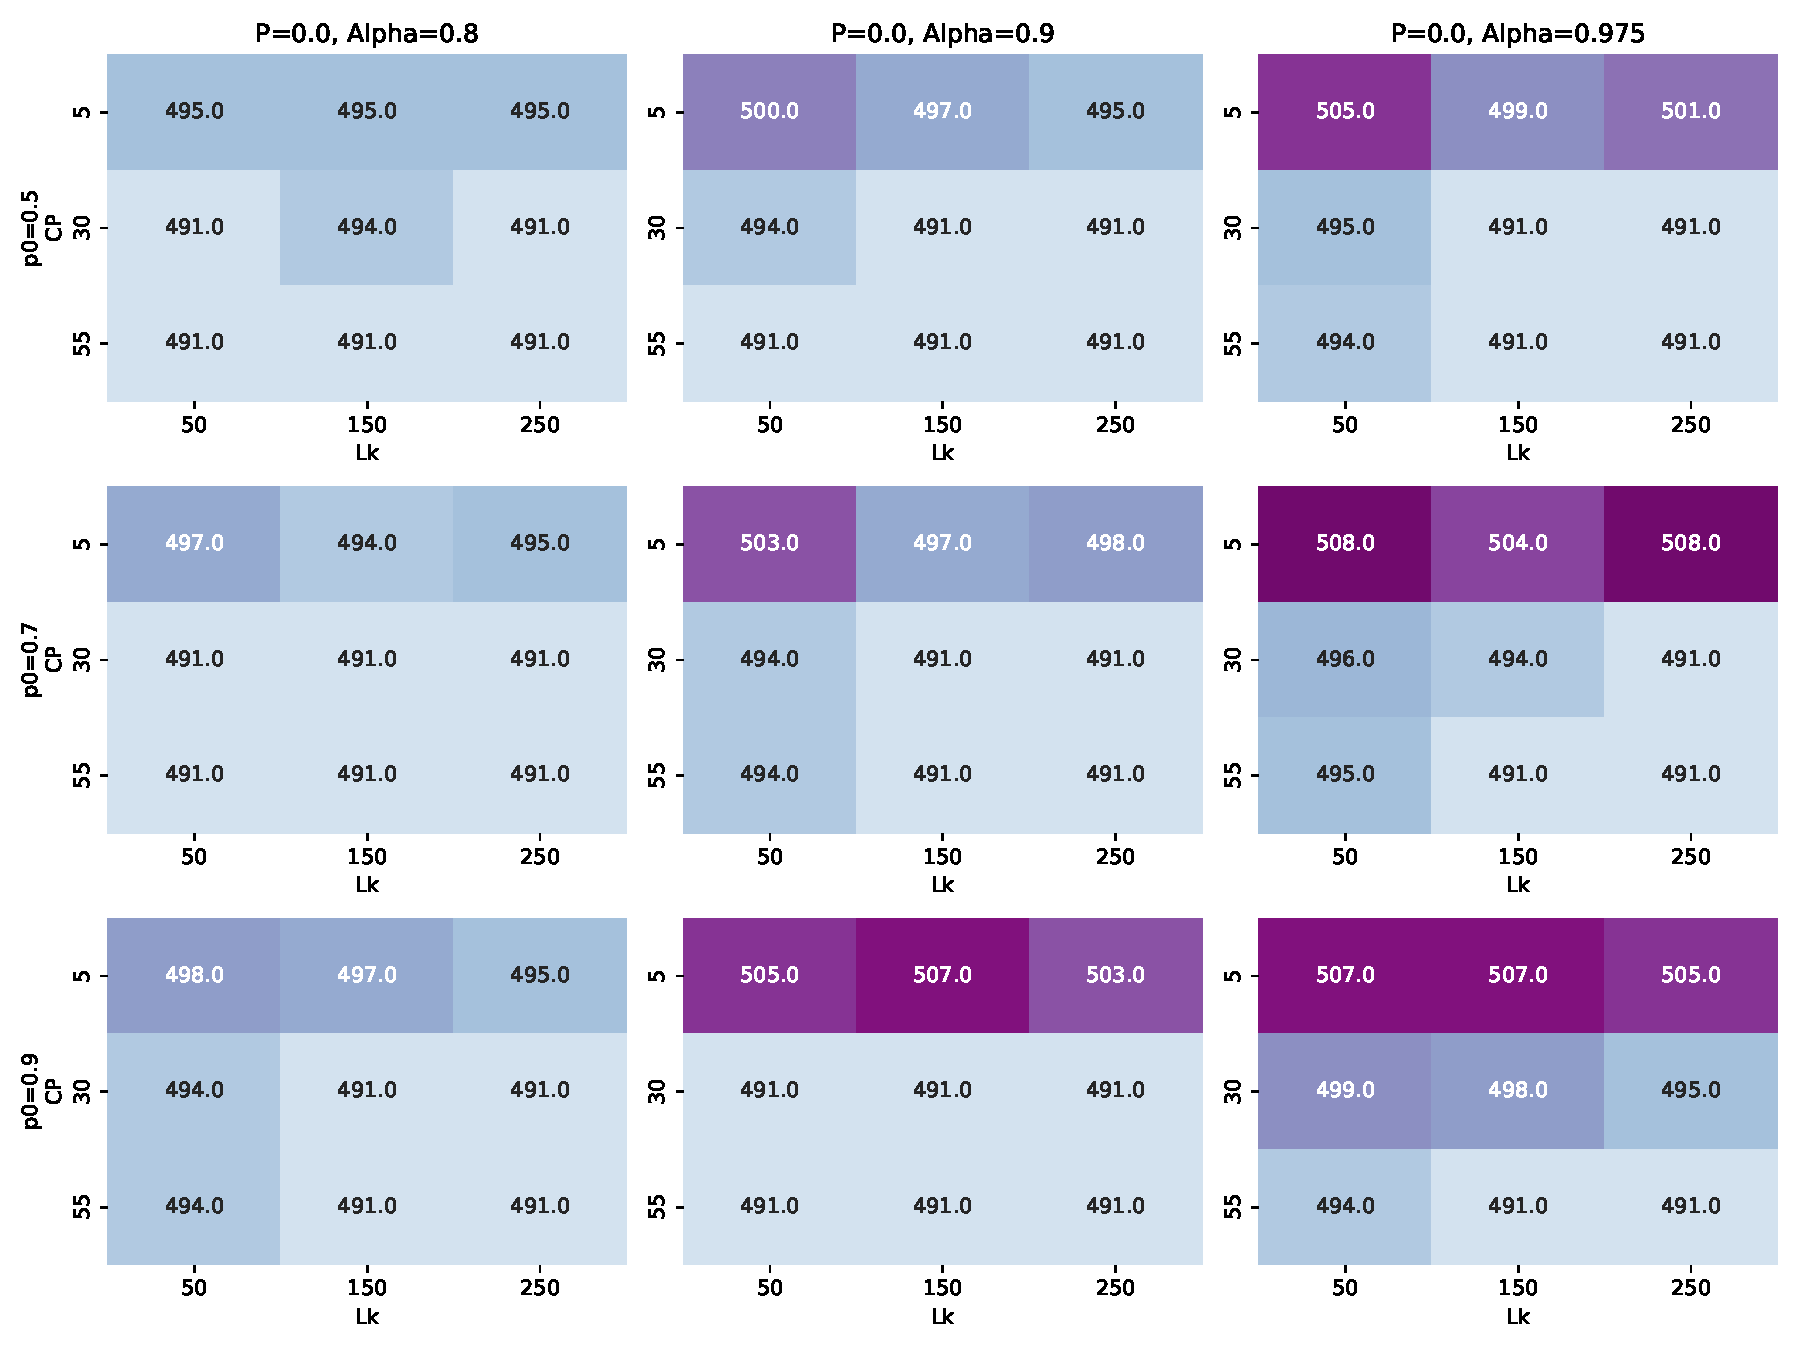
\includegraphics[width = \textwidth]{P1M2_GV_REVTT_best}
		\caption{Melhor \textit{makespan}}
		\label{fig:P1M2_GV_REVTT_best}
	\end{subfigure}
	\begin{subfigure}{0.49\textwidth}
	\centering
		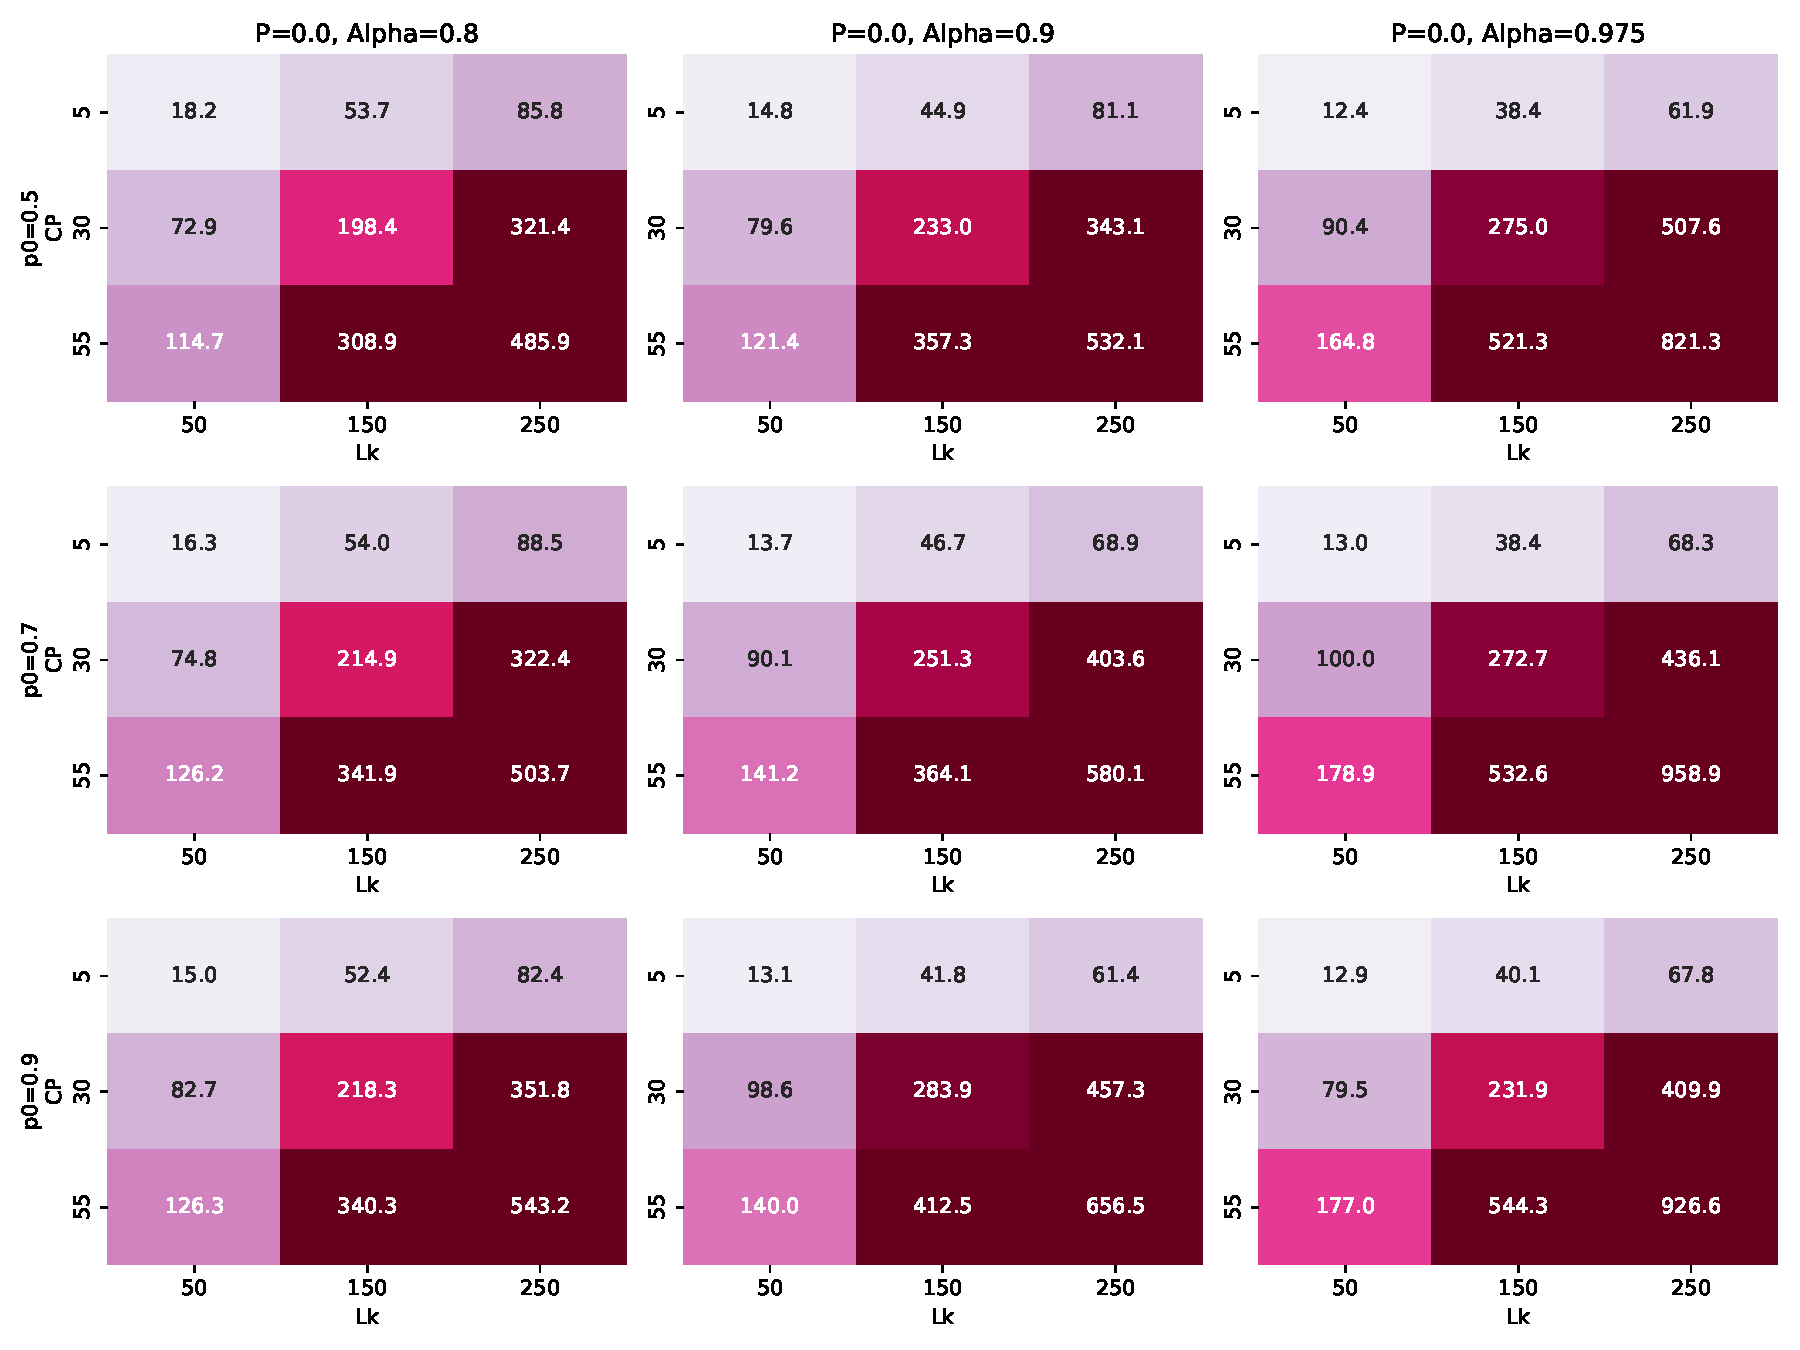
\includegraphics[width = \textwidth]{P1M2_GV_REVTT_runtime}
		\caption{Tempo de computação total}
		\label{fig:P1M2_GV_REVTT_runtime}
	\end{subfigure}
	\caption{Impacto dos níveis das variáveis sobre o valor da função objetivo e do tempo computacional para o modelo 3 com \textit{enhanced left shifting}.}
	\label{fig:P1M2_GV_REVTT_alt}
\end{figure}

\section{Problema do número de trabalhos}

\begin{figure}[H]
	\centering
	\begin{subfigure}{0.49\textwidth}
	\centering
		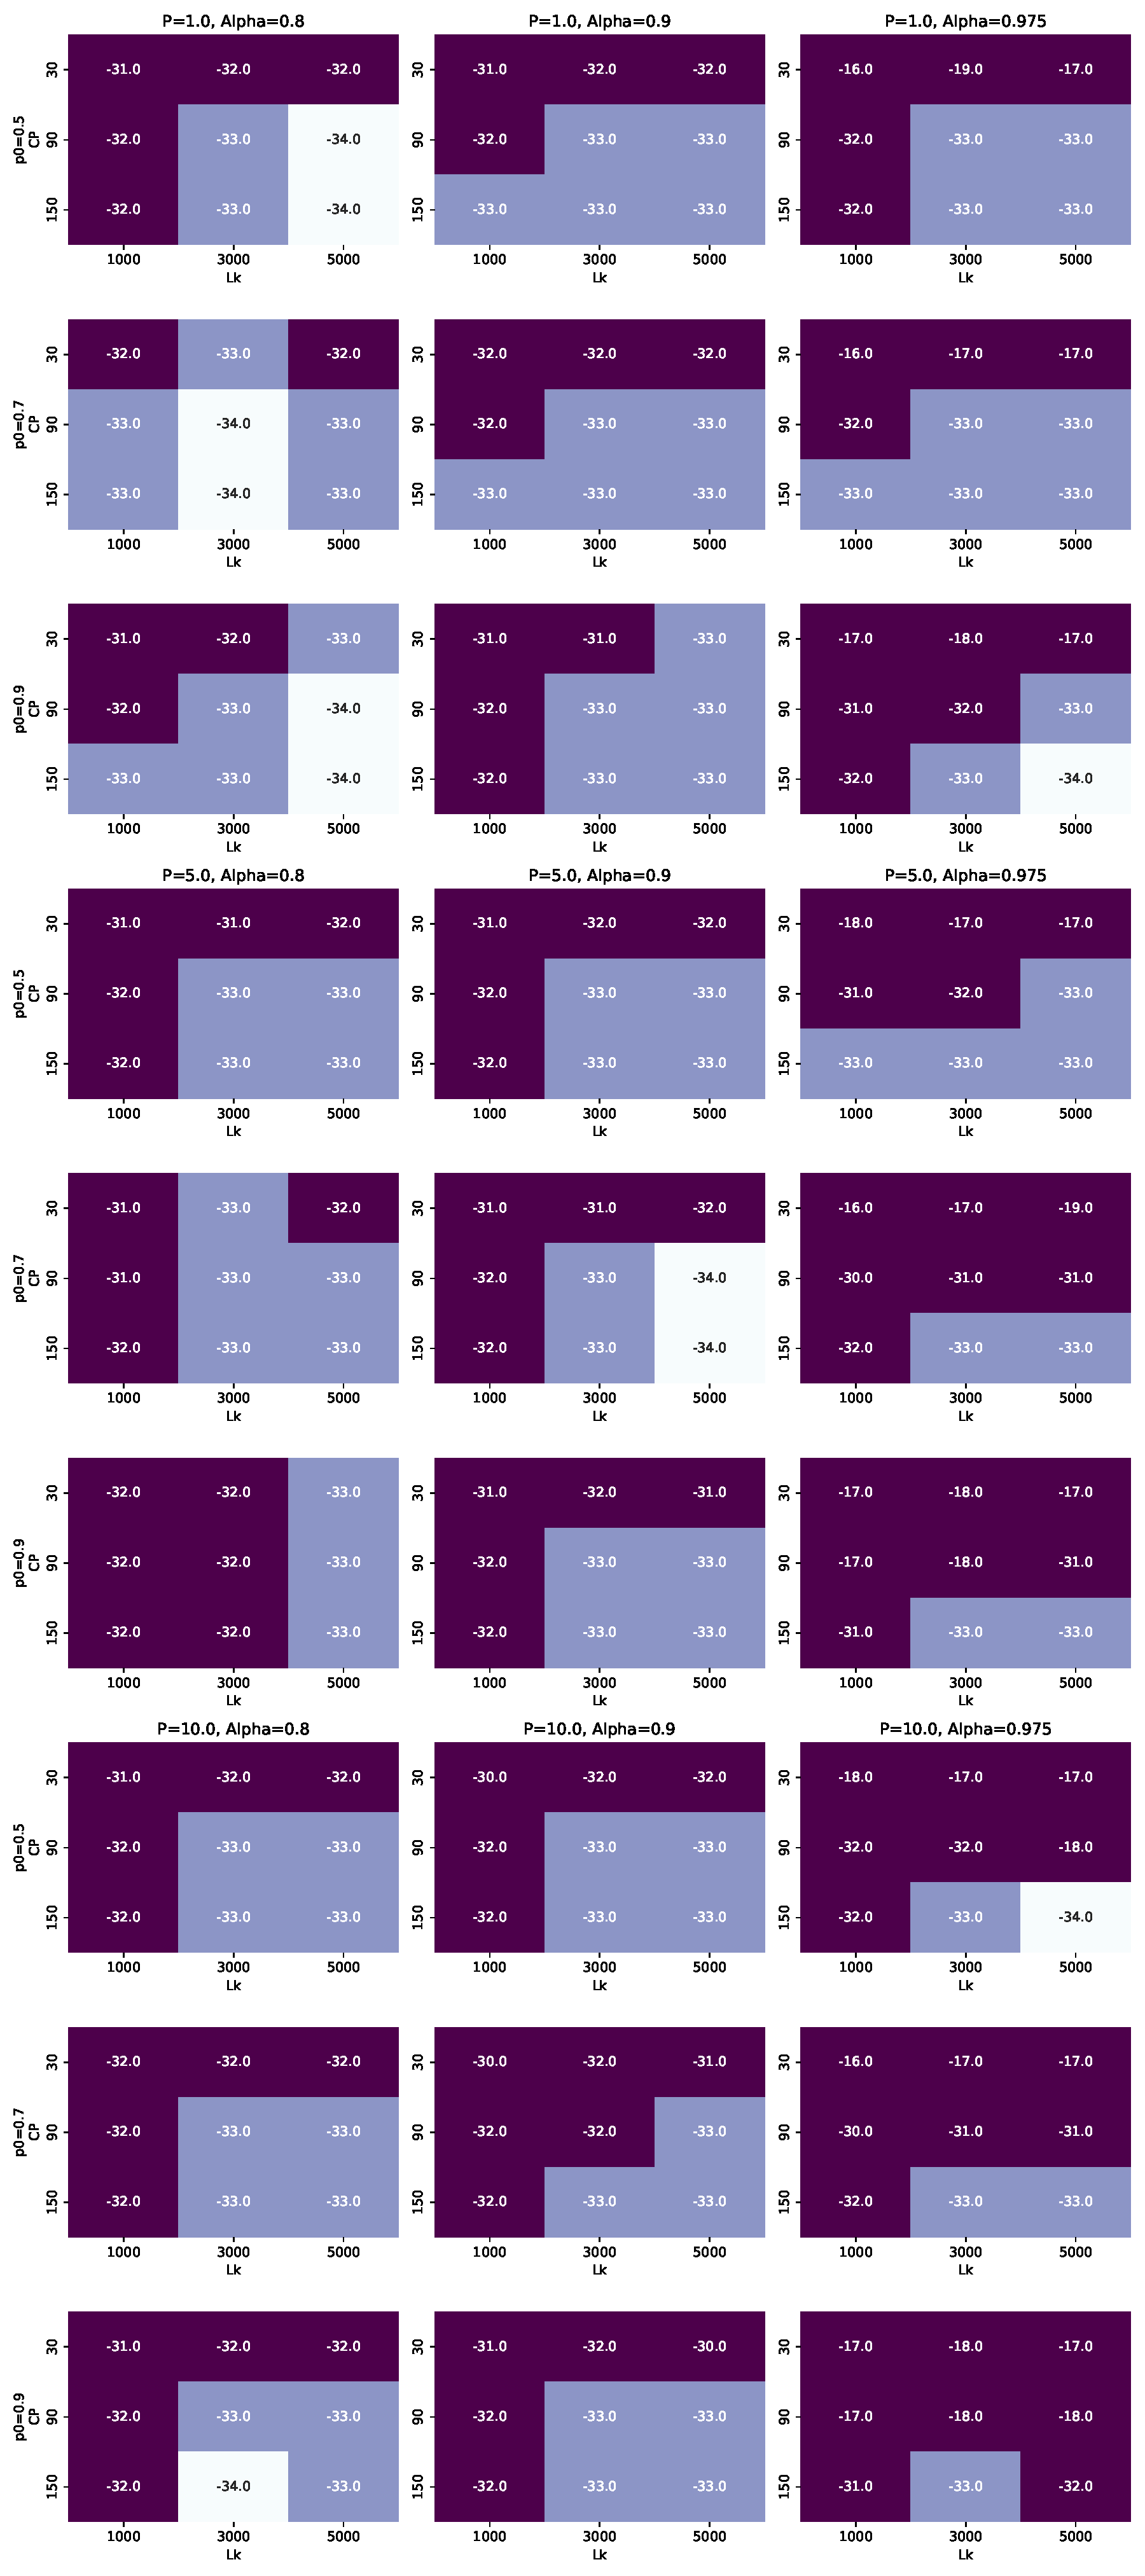
\includegraphics[width = \textwidth]{P2M1_NNGV_best}
		\caption{Melhor número de trabalhos}
		\label{fig:P2M1_NNGV_best}
	\end{subfigure}
	\begin{subfigure}{0.49\textwidth}
	\centering
		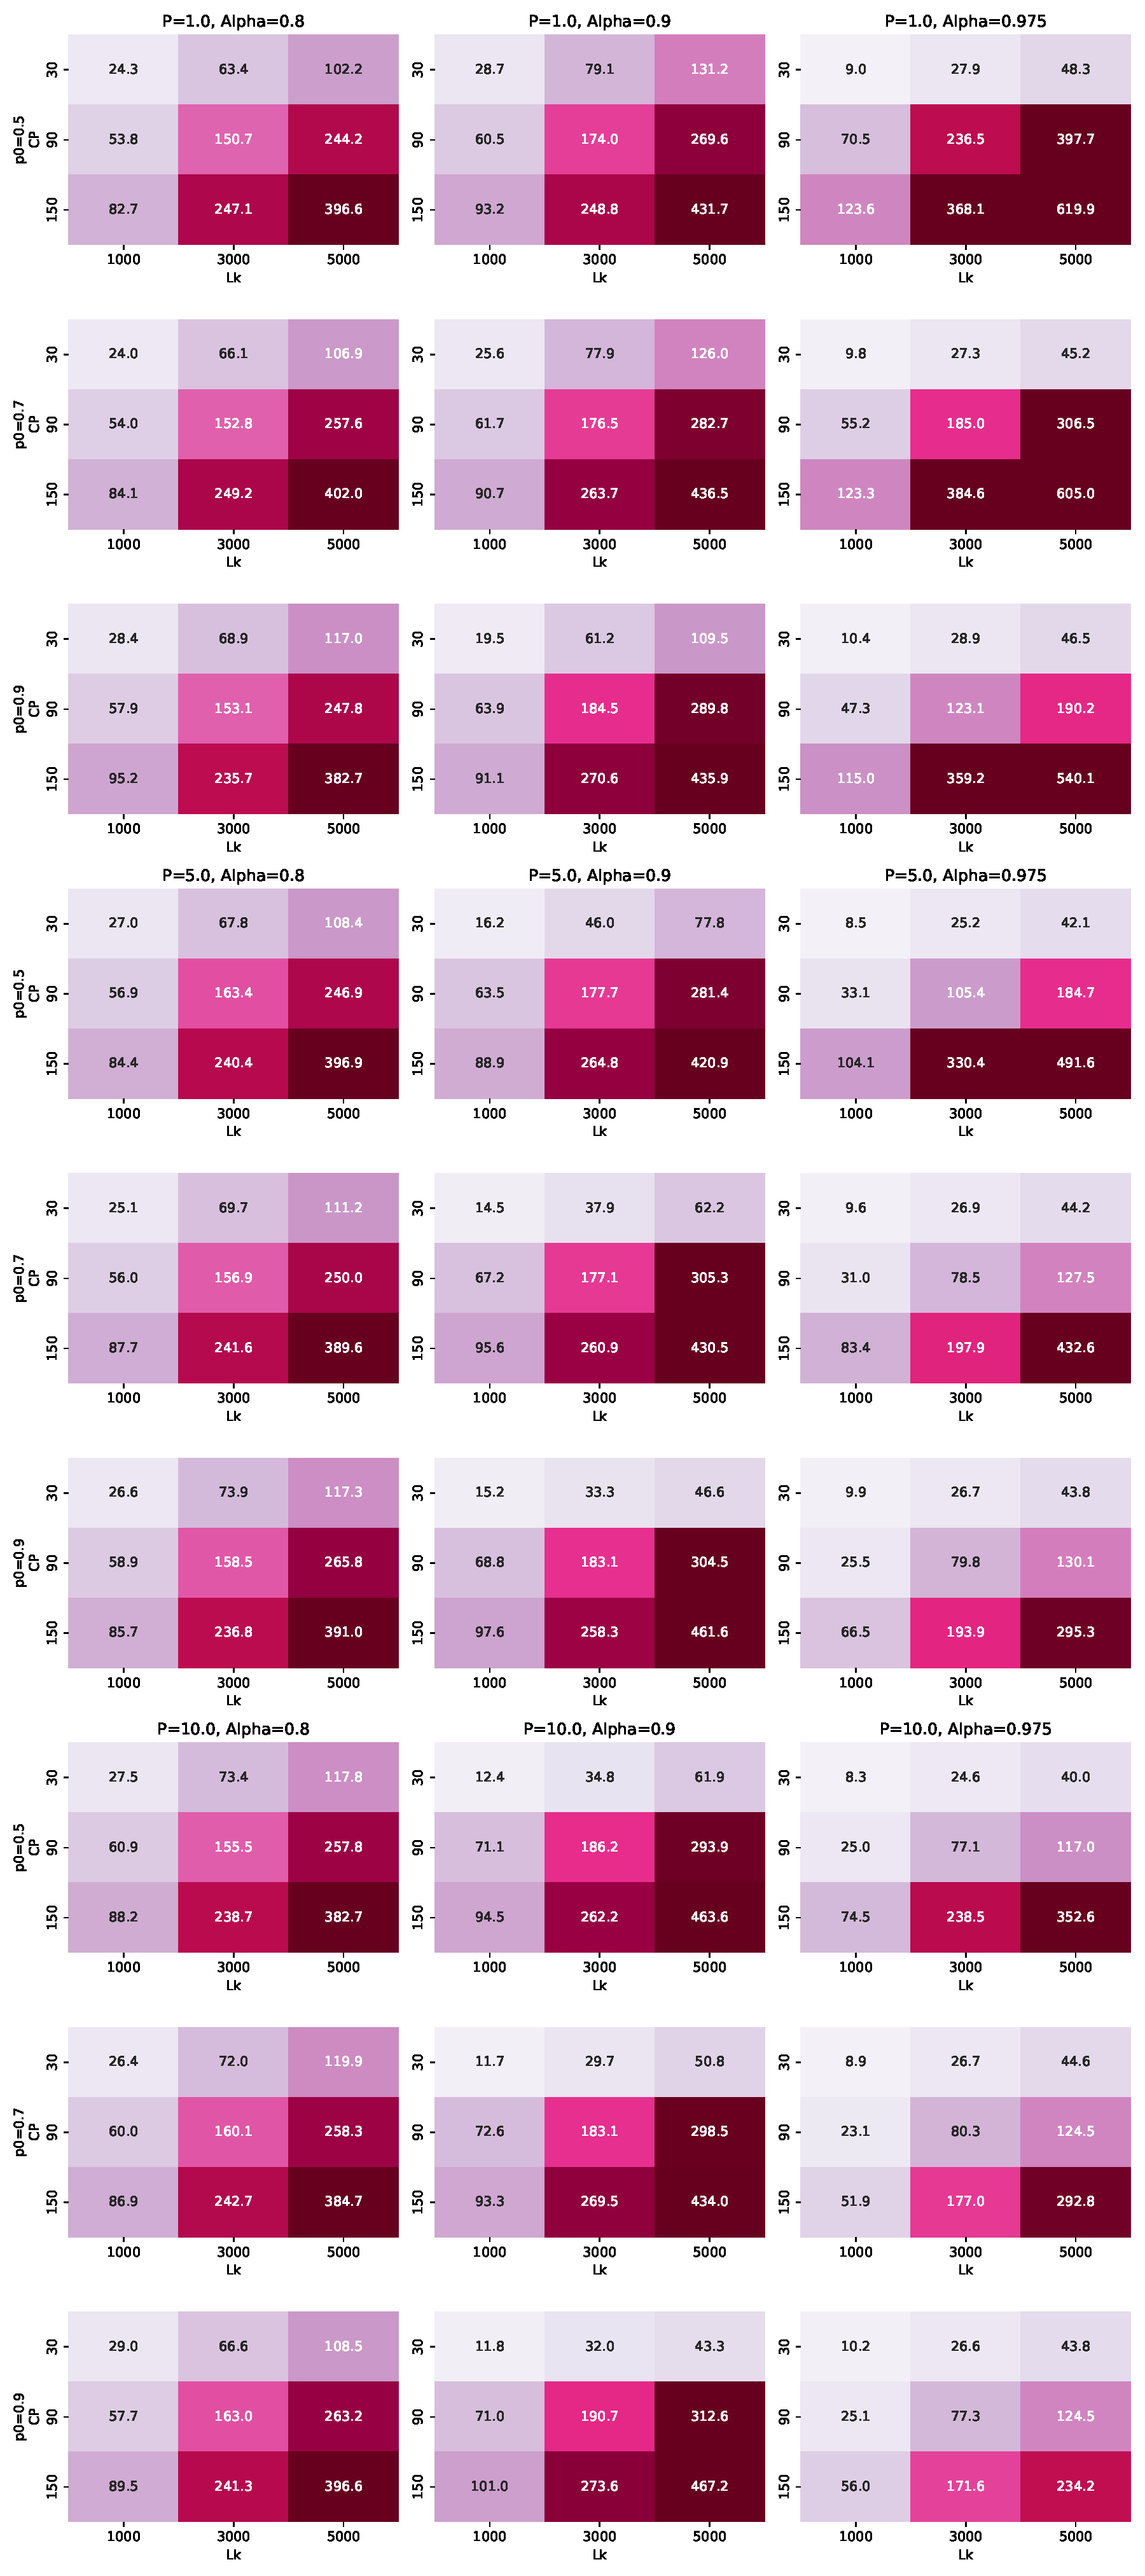
\includegraphics[width = \textwidth]{P2M1_NNGV_runtime}
		\caption{Tempo de computação total}
		\label{fig:P2M1_NNGV_runtime}
	\end{subfigure}
	\caption{Impacto dos níveis das variáveis sobre o valor da função objetivo e do tempo computacional para o modelo 1.}
	\label{fig:P2M1_NNGV_alt}
\end{figure}